
\documentclass[a4paper,12pt,twoside]{exam}
\usepackage{acn-particlestyle}
\usepackage{acn-scientific}
\usepackage{acn-questions}

\usetikzlibrary{circuits.ee.IEC}

\usepackage{color}
\definecolor{heberblue}{rgb}{0,0,1}

\newcounter{saveenumi}


\begin{document}

\begin{titlepage}

\begin{minipage}{0.2\textwidth}
\includegraphics[width=0.8\textwidth]{img/heber.jpg}
\end{minipage}
\hspace{0.05\textwidth}
\begin{minipage}{0.7\textwidth}
\begin{Huge}\textcolor{heberblue}{\textbf{Bishop Heber High School}}\end{Huge}
\end{minipage}\\

\bfseries

\vspace{6em}

\begin{Huge}Practical Physics\end{Huge}\\
\indent \Large Sixth form\\

Draft version\\


\begin{minipage}{0.45\textwidth}
\hfill
%\includegraphics[width=0.8\textwidth]{img/doubleslit.jpg} 
\hfill	
\end{minipage}
\begin{minipage}{0.45\textwidth}
%\footnotesize{{
%A modern-day replica of Thomas Young's double-slit experiment, a classic experimental demonstration of the wave nature of light. The interference patterns shown are observed when a coherent beam from either a red helium-neon laser (\SI{632.8}{nm}, top), or a green helium-neon laser (\SI{543.4}{nm}, bottom), is used to illuminate two \SI{25}{\micro\meter} wide slits which are \SI{75}{\micro\meter} apart. The two diffraction patterns are observed at the same distance from the double-slit. Note that the fringe spacing is smaller for shorter (green) wavelength.
%}}
\end{minipage}
\begin{flushright}
%\rmfamily{\small{GIPHOTOSTOCK / SCIENCE PHOTO LIBRARY}}
\end{flushright}

\vfill

\begin{minipage}{0.5\textwidth}
Name:\\
\hrule
\vspace{0.5em} Form: \\
\hrule
\vspace{0.5em} Set: \\
\hrule
\end{minipage}

\thispagestyle{empty}
%\enlargethispage{4cm}
	
\end{titlepage}

\newpage
\thispagestyle{empty}

\vspace*{4cm}

\begin{center}
\fbox{
\begin{minipage}{0.65\textwidth}
\vspace*{1em}
\begin{center}
\includegraphics[width=0.3\textwidth]{by-nc-sa.png}
\end{center}
\raggedright

This work by A.C. Norman is licensed under a Creative Commons
Attribution-NonCommercial-ShareAlike License.

{\footnotesize\texttt{http://creativecommons.org/licenses/by-nc-sa/3.0/}}\\

\vspace{1em}

Non-commercial uses are thus permitted without any
further permission from the copyright owner.\\

\vspace{1em}

%Permissions beyond the scope of this license are
%administered by the author. Information on how
%to request permission may be found at:
%http://www.randomhouse.com/about/
%permissions.html
\end{minipage}
}
\end{center}

\newpage

%
\section*{Errors}

In practical work in AS and A2 physics, you should be prepared to
\begin{itemize}
\item identify the source of uncertainties in an experiment.
\item calculate the fractional or percentage error from the size of the measurement and the absolute error on it.
\item combine the uncertainties of different measurements when you evaluate something which depends on a number of quantities. It is very unlikely that you will have to do a full calculation of the total error, but you may be asked, for example, to identify which individual measurement contributes the biggest uncertainty.
\end{itemize}

\subsection*{Sources of uncertainty and absolute errors}

Any measurement has a statistical uncertainty associated with it. It is generally a combination of both the reading error on a measuring instrument and the uncertainty to do with the way you are performing the measurement. For example, the reading error on a \SI{1}{m} ruler is at best \SI{0.5}{mm}. If you are using it to measure the depression of another ruler, you might reasonably assign a total uncertainty of \SI{3}{mm}, to account for the fact that you may not have the measuring ruler absolutely vertical. An error of this kind is an absolute error, and has the dimension of the quantity you are measuring.

Systematic errors may also be built in to the experiment, for example the ruler above may have an actual length of say \SI{99}{cm} when you have assumed to be \SI{1}{m}, or an ammeter may show a non-zero reading when disconnected from an electric circuit. Such uncertainties may not alter the reliability of your readings, but they may well affect the accuracy of a calculated quantity.

\subsection*{Fractional or percentage errors}

These are dimensionless and are calculated using the formula
\[\text{fractional error} =  \frac{\text{absolute error}}{\text{size of measurement}}.\]

\subsection*{Combination of errors}

\begin{itemize}
\item If you make two measurements of the same type $x$ and $y$, for example the length and breadth of a table, then
absolute error on the sum $x+y$ or difference $x-y$ of $x$ and $y$ is equal to the sum of absolute errors on $x$ and $y$.
\item If you make measurements of any two quantities $x$ and $y$, then 
fractional error on the product $xy$ or quotient $x/y$ is equal to the sum of fractional errors on $x$ and $y$.
\item If a power law holds
\[\text{fractional error on $x^{k}$}  = k \times \text{fractional error on $x$}.\]
\end{itemize}

%Example 1 . A rectangular table is measured to have length 2.5m � 2mm and breadth 0.5m � 2mm. Find the absolute error on the %circumference and the area.

%Answer	Absolute error on circumference = sum of absolute errors on four sides = 4 ? 2mm = 8mm
%Fractional error on area = 
%fractional area on length + fractional area on breadth = 2mm/2.5m +  2mm/0.5m =  0.5 %.
%Absolute error on area = 0.5 % ? (2.5 m ? 0.5 m) =  60 cm2.

%Example 2. A simple pendulum is measured to be 50cm � 5mm in length. Ten swings are timed to take 14.0 s � 0.2s. Which measurement contributes a larger uncertainty to a value of g derived from this experiment ?  What is the absolute error on g? 

%Answer	T = 2??(l/g) therefore g = 4?2l/T2.   
%Fractional error on g = 
%fractional error on l + 2 ? fractional error on T = 0.5/50  + 2 ? 0.02/1.40 = 1% + 3% = 4%.
%Therefore the error on the period has a far greater contribution than that on the length. Note that if only one swing was timed, the fractional error on the period would be ten times as large.
%Absolute error on g = fractional error ? size of g = 4% ? 10.1 ms-2   =  0.4 ms-2. 
%Although the value of g is greater than the true value of 9.81 ms-2, the measurement is in agreement within the error, as it should be if the errors have been realistically assessed. 

%Error on a count

%Any count of a number of occurrences e.g. the number of clicks of a Geiger counter in a period of time has an uncertainty associated with it. If there are N counts, then the absolute error is of size ?N. Thus the absolute error increases with N, but the fractional error =   ?N / N = 1/?N gets smaller. Therefore it is desirable to make the number of counts as big as possible.
%E.g. if a Geiger counter records 100 background counts over a period of 1 minute, the percentage error is 100% ? (1/?100) = 10%. 
%If the same measurement is made over 4 minutes, we expect a percentage error of 100% ? (1/?400) = 5%.

\newpage
\section*{Determining relationships by plotting graphs}

When a certain relationship exists between two variables $y$ and $x$, its form can sometimes be determined by plotting a suitable graph. You should be familiar with the following cases.

\subsection*{Linear}

If $y = mx + c$ a graph of $y$ against $x$ should be a straight line with gradient $m$ and $y$-intercept $c$.\\
NB $y$ is only proportional to $x$ if $c = 0$.

\subsection*{Exponential}

If  $y = Ae^{-mx}$ , where $A$ is a constant, then taking natural logs of both sides gives
\[ \ln y = \ln A + \ln(e^{-mx}) = \ln A - mx.\]
Hence a graph of $\ln y$ against $x$ should be a straight line of gradient $-m$ and intercept $\ln A$.\\
Examples of such relationships are found in radioactive decay and in electric circuits containing capacitors.

\subsection*{Polynomial}

If  $y = Ax^{m}$  , then taking natural logs of both sides gives
 \[\ln y = \ln A + \ln(x^{m}) = \ln A +  m\ln x.\]
Hence a graph of $\ln y$ against $\ln x$ should be  a straight line of gradient $m$ and intercept $\ln A$.\\
Examples include the variation of the period of a simple pendulum with length ($m = 0.5$) and the energy stored in a stretched spring with extension ($m = 2$).

\section*{Errors obtained from graphs}

When it is believed that a linear relationship exists between two quantities plotted on a graph, a straight line of best fit should be drawn through the points, which passes as close to all the points as possible. 

You can draw error bars for each point so that the length of the line on either side of the point represents the absolute error you have assigned to the individual measurements. The line of best fit should pass through about two-thirds of the error bars, if you have assessed the errors realistically (and if a linear relationship holds).

It is common to extract the gradient or the intercept since they often correspond to something interesting. You can evaluate the error on them by drawing another fit line, making it as steep or shallow as possible, so that it still passes through the error bars. The difference between the values so obtained for the gradient and intercept, and those of the best-fit line correspond to the absolute errors.


\normalsize

\newpage
\section*{Index}
%\setlength{\extrarowheight}{0.3cm}
\renewcommand{\arraystretch}{1.6}
\begin{center}
\begin{tabular}{|l|c|p{2.5cm}|p{2cm}|c|}
\hline
\multicolumn{1}{|c|}{\bf Experiment} & \multicolumn{1}{|c|}{\bf Page} & \multicolumn{1}{|c|}{\bf Date} & \multicolumn{1}{|c|}{\bf Mark}\\
\hline
\ref{photoelectric} - Photoelectric effect & \pageref{photoelectric} & & \\
\hline
\end{tabular}
\renewcommand{\arraystretch}{1}
\end{center}

\cleardoublepage

\section{The Photoelectric effect}
\label{photoelectric}

In quantum theory, light exists as a stream of photons, each with energy $hf$, where $h$ is Planck's constant and $f$ is the frequency of the light.
\[E_{\text{photon}}=hf=\frac{hc}{\lambda},\]
where $\lambda$ is the wavelength of the light.

When the light is incident on a metal surface, an electron in the surface may absorb a photon, and therefore its energy.  The electron is held in the surface by an attractive force, which needs an amount of energy called the work function $\phi$ to be overcome.  It follows that an electron will be emitted if it absorbs a photon with energy greater then the work function.  Any excess energy will become kinetic energy of the electron.

This can be written in Einstein's photoelectric equation:
\[hf=\phi+E_{k}.\]

A (negative) voltage, called the stopping voltage $V_{S}$ can be applied to stop electrons leaving the surface.

\subsection{Setup}

You need to use a d.c. power supply of \SI{6}{V}, a voltmeter and a milliammeter.  All of the LEDs you will use are in a specially-made box for this experiment, which you need to connect up with the voltage supply and measuring apparatus as shown on the box.  The circuit is as follows:\\

\begin{minipage}{0.6\textwidth}
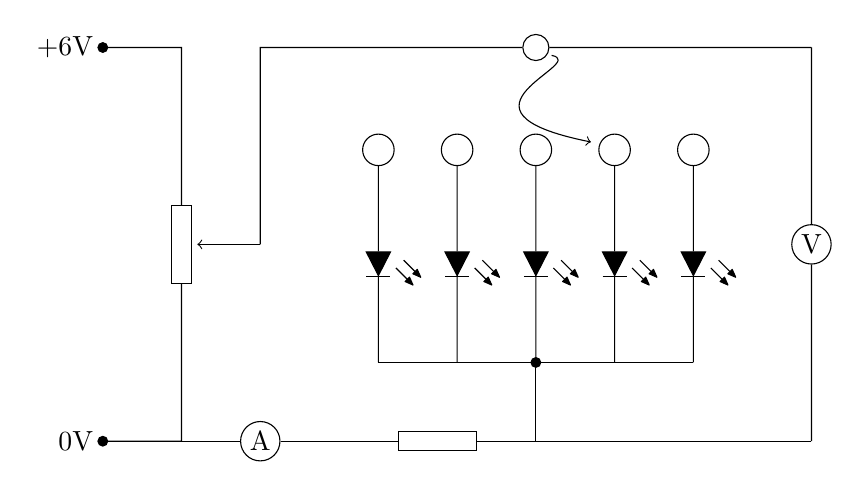
\begin{tikzpicture}[circuit ee IEC,set diode graphic=var diode IEC graphic]
\draw (0,0) node[contact]{} node[anchor=east]{\SI{0}{V}} to (1,0) to [resistor] (1,5) to (0,5) node{} node[anchor=east]{\SI{+6}{V}} node[contact]{};
\draw (0,0) to (1,0) to [circuit handle symbol={draw,shape=circle,label=center:{A},minimum size=5mm}] (3,0) node{} to [resistor] (5.5,0) node{} to (9,0);
\draw (9,0) to [circuit handle symbol={draw,shape=circle,label=center:{V},minimum size=5mm}] (9,5);
\draw (9,5) to [circuit handle symbol={draw,shape=circle,minimum size=2mm}] (2,5) to (2,2.5);
\draw[->] (2,2.5)--(1.2,2.5);
\draw (5.5,0) to (5.5,1) node[contact]{};
\draw (3.5,1) to (7.5,1);
\foreach \diode in {0,1,...,4}
{
\draw (3.5+\diode,3.5) to [diode={light emitting}] (3.5+\diode,1);
\draw (3.5+\diode,3.7) circle (0.2);
}
\draw[->] (5.7,4.9) .. controls (6.2,4.8) and (4.2,4.2) .. (6.2,3.8);
\end{tikzpicture}
\end{minipage}
\begin{minipage}{0.35\textwidth}
Some data on the LEDs from the manufacturer is below:\\

\renewcommand{\arraystretch}{1}
\begin{tabular}{lcc}
\hline
Colour & $\lambda$/nm & $I_{\text{max}}$/mA\\
\hline
Red & 700 & 25\\
Orange & 627 & 30\\
Yellow & 590 & 30\\
Green & 565 & 25\\
Blue & 430 & 30\\
\hline
\end{tabular}
\renewcommand{\arraystretch}{2}
\end{minipage}

\subsection{Measurements}
For each LED, you need to take several readings of current and voltage (which will allow you to plot a current-voltage characteristic), by increasing the voltage from zero until the current reaches the manufacturer's recommended maximum current (and no further).

\begin{minipage}{0.3\textwidth}
\begin{tabular}{|p{2cm}|p{2cm}|}
\hline
\multicolumn{1}{|c|}{$V$/V} & \multicolumn{1}{|c|}{$I$/}\\
\hline
&\\
\hline
&\\
\hline
& \\
\hline
& \\
\hline
& \\
\hline
& \\
\hline
\end{tabular}
\end{minipage}
\begin{minipage}{0.3\textwidth}
\begin{tabular}{|p{2cm}|p{2cm}|}
\hline
\multicolumn{1}{|c|}{$V$/V} & \multicolumn{1}{|c|}{$I$/}\\
\hline
&\\
\hline
&\\
\hline
& \\
\hline
& \\
\hline
& \\
\hline
& \\
\hline
\end{tabular}
\end{minipage}
\begin{minipage}{0.3\textwidth}
\begin{tabular}{|p{2cm}|p{2cm}|}
\hline
\multicolumn{1}{|c|}{$V$/V} & \multicolumn{1}{|c|}{$I$/}\\
\hline
&\\
\hline
&\\
\hline
& \\
\hline
& \\
\hline
& \\
\hline
& \\
\hline
\end{tabular}
\end{minipage}

\begin{minipage}{0.3\textwidth}
\begin{tabular}{|p{2cm}|p{2cm}|}
\hline
\multicolumn{1}{|c|}{$V$/V} & \multicolumn{1}{|c|}{$I$/}\\
\hline
&\\
\hline
&\\
\hline
& \\
\hline
& \\
\hline
& \\
\hline
& \\
\hline
\end{tabular}
\end{minipage}
\begin{minipage}{0.3\textwidth}
\begin{tabular}{|p{2cm}|p{2cm}|}
\hline
\multicolumn{1}{|c|}{$V$/V} & \multicolumn{1}{|c|}{$I$/}\\
\hline
&\\
\hline
&\\
\hline
& \\
\hline
& \\
\hline
& \\
\hline
& \\
\hline
\end{tabular}
\end{minipage}
\begin{minipage}{0.3\textwidth}
\begin{tabular}{|p{2cm}|p{2cm}|}
\hline
\multicolumn{1}{|c|}{$V$/V} & \multicolumn{1}{|c|}{$I$/}\\
\hline
&\\
\hline
&\\
\hline
& \\
\hline
& \\
\hline
& \\
\hline
& \\
\hline
\end{tabular}
\end{minipage}

\begin{questions}
\question Plot the current-voltage characteristics for all of the LEDs on the {\bf same} graph, with voltage on the $x$-axis and current on the $y$-axis (take care to label the curves!)  On this graph, you need to extrapolate each curve down to the $x$-axis to find the voltage at which current first starts to flow, and light photons start to be emitted.  Use this to fill in the table below.

\begin{center}
\begin{tabular}{|l|c|p{2cm}|p{2cm}|}
\hline
Colour & $\lambda$ &  \multicolumn{1}{|c|}{$1/\lambda$ } & \multicolumn{1}{|c|}{$V_{\text{min}}$}\\
 & / nm & \multicolumn{1}{|c|}{/ \ldots} & \multicolumn{1}{|c|}{/ V} \\
\hline
Red & 700 & &\\
\hline
Orange & 627 & &\\
\hline
Yellow & 590 & &\\
\hline
Green & 565 & &\\
\hline
Blue & 430 & &\\
\hline
\end{tabular}
\end{center}

\question Now plot a second graph, this time of the minimum voltage for light emission on the $y$-axis against the LED wavelength on the $x$-axis.

\question Work out the gradient, showing your working on the graph. \answerline

According to theory, your gradient $G$ is related to Planck's constant by $h=eG/c$, where $e$ is the electronic charge, \SI{1.6e-19}{C}, and $c$ is the speed of light, \SI{3e8}{m.s^{-1}}.

\question What value does your experiment give for $h$? \answerline

\question Comment briefly on this value, and on the quality of your data, on your second graph. What do you think were the biggest sources of error in this experiment?
\end{questions}
%graph paper incl.

\end{document}
